% !Mode:: "TeX:UTF-8"
\chapter{引言}
\mingyan{满纸荒唐言,一把辛酸泪!都云作者痴,谁解其中味?}{曹雪芹}

本模板完全由国防科技大学的模板改来,初次制作,不足之处在所难免,欢迎提供建议,在此感谢Liubenyuan同学,模板里很多地方对我帮助很大。模板详细说明基本上可以参考nudtpaper-2.2.pdf。

我还是比较满意我做的两个封面\footnote{论文封面和任务书封面},你只需在thesis.tex中仿照模板填上相关数据即可。由于我们学校的论文要求里面也没说正文版面大小,我就根据以前一个学姐的论文测量出页边距,页眉,页脚等一些参数,做的这个。算是基本满足学校的要求了,就看学校收不收了。
\section{本模板的一些使用说明}
任务书及开题报告本来是不想做的,有些难度。但真是皇天不负有心人,终于让我在天津大学的模板里找到了这个东西,花了一个下午做出了那些表格。当然你也可以不用我做的那个,将\latexinline|% !Mode:: "TeX:UTF-8"
\pagestyle{empty}
\vspace*{1ex}
\myoverlay%为当前页添加边框
{\cusong\sihao\hspace*{-2em} 一、设计内容}
     \begin{enumerate}
     \item 准备了解有关导航以及导航系统的特点、应用前景。
     \item 准备对导航系统中常用的惯导器件—陀螺仪进行说明。
     \item 准备对提高导航信号测量精度所用到的滤波技术进行软件仿真。
     \item 准备分析比较各种滤波信号,并得出相应结论。
     \end{enumerate}

\myhline%划横线
{\cusong\sihao 二、设计原始资料}
     \begin{enumerate}
     \item 导航系统的相关资料
     \item 惯导器件基础教程及有关书籍
     \item 卡尔曼滤波、神经网络相关资料
     \item \Matlab{}软件教程及相关资料
     \end{enumerate}

\myhline%划横线
{\cusong\sihao 三、设计完成后提交的文件和图表}
     \begin{enumerate}
     \item 计算说明书部分
     \begin{enumerate}
     \item 卡尔曼滤波、扩展卡尔曼滤波以及无迹卡尔曼滤波对比仿真图
     \item 各种滤波算法应用范围对比表
     \end{enumerate}
     \item 图纸部分
     \begin{enumerate}
     \item 几种惯性导航系统原理框图
     \item 改进卡尔曼滤波效果仿真图
     \item 卡尔曼滤波、扩展卡尔曼滤波以及无迹卡尔曼滤波效果仿真比较图
     \end{enumerate}
     \end{enumerate}

\myhline
{\cusong\sihao 四、毕业设计进程安排}

          \vspace{2em}
          {\heiti 序号\hspace{5em}设计各阶段名称\hspace{9em}日期(教学周)}

          {\hspace{0.5em}1\hspace{3em}阅读相关书籍,完成开题报告\hspace{4em}3月1 日--3月14日(第1--2周)}

          {\hspace{0.5em}2\hspace{3em}准备了解常见导航系统的相关知识\hspace{2em}3月15 日--3月28日(第3--4周)}

           {\hspace{0.5em}3\hspace{3em}研究导航系统中较常见的惯导器件\hspace{2em}3月29日--4月11日(第5--6周)}

           {\hspace{0.5em}4\hspace{3em}学习导航系统中几种常用滤波技术\hspace{2em}4月12日--5月9日(第7--10周)}

           {\hspace{0.5em}5\hspace{3em}准备对滤波算法进行仿真比较\hspace{4em}5月10日--5月16日(第11周)}

           {\hspace{0.5em}6\hspace{3em}撰写毕业论文\hspace{11em}5月17日--6月10日(第12--14周)}

\myhline
{\cusong\sihao 五、主要参考资料}
\begin{bibList}
\item 于国强. 导航与定位. 北京:国防工业出版社.2000.2:1.
\item 邓正隆. 惯性导航原理.哈尔滨:哈尔滨工业大学出版社.1994.1:1-2,2-5.
\item 袁建平. 卫星导航原理与应用.中国宇航出版社.2003 第一版:23-24.
\item 秦永元. 惯性导航.北京:中国科学出版社.2006:1-5.
\item 陈开权. 惯性导航的理论基础[J]. 北京: 水雷战与舰船防护,2003(1):76-90.
\item 付梦印,邓志红,张继伟.Kalman 滤波理论及其在导航中的应用.北京:科学出版社.2003.
\end{bibList}

%%%%%%%%%%%%%%%%%%%  长安大学毕业设计(论文)开题报告表  %%%%%%%%%%%%%%%%%%%%%%%
\newpage
\markboth{长安大学毕业设计(论文)开题报告表}{长安大学毕业设计(论文)开题报告表}
\pdfbookmark[0]{长安大学毕业设计(论文)开题报告表}{creport}
\begin{center}
\hei\sanhao{长安大学毕业设计(论文)开题报告表}
\end{center}
\begin{table}[h]
  \centering\xiaosi
  \begin{tabularx}{\textwidth}{|c|p{0.15\textwidth}|c|X|c|X|}
     \hline
     课题名称 & \multicolumn{5}{c|}{TeX惯性器件精度提高实现方法} \\ \hline
     课题来源 & \centering {自选课题} & 课题类型 & \centering {工程设计} & 指导教师 & \centering {CTeX} \tabularnewline \hline
     学生姓名 & \centering {Tsingber  Lee} & 学\hspace*{24bp}号 & \centering {2403000001} & 专\hspace*{24bp}业 & \centering {电子信息工程} \tabularnewline \hline
   \end{tabularx}
      \centering\xiaosi
\end{table}
%%%%%%%%%%%%%%%%%画图区%%%%%%%%%%%%%%%%%
\setlength{\unitlength}{1mm}
\noindent\begin{picture}(0.1,0)
\multiput(0.1,0)(160.8,0){2}{\line(0,-1){188}}
\multiput(0.1,0)(160.8,0){2}{\line(0,1){9.3}}
\put(0.1,-188){\line(1,0){160.8}}
\end{picture}
%%%%%%%%%%%%%%%%%%%%%%%%%%%%%%%%%%
     {  {\heiti (一)课题意义:}

 由半导体工业中的微细加工技术与机械工业中的微型机械加工技术结合而产生并逐渐发展起来的微电子机械系统(MEMS: Microelectro Mechanical Sys2tem) 是微米、纳米电子学的重要领域,是一项极具发展前景的军民两用高技术,它的出现,将引发一场新的技术革命。

微电子机械系统涉及到微电子学、自动控制、光学、气动力学、流体力学和声学磁学等多种领域,可以说是一门多学科的综合技术。它研究的主要内容包括微型传感器、微型执行器和复杂的微系统。提高MEMS加速计传感器的精度具有重要意义。

{\noindent\heiti (二)国内外发展状况:}

(1)国外概况:

MEMS 技术的开发始于20 世纪60 年代,其迅速发展是在20世纪80年代末期,由MEMS技术的迅速发展,在1987年便决定把MEMS从IEEE国际微机器人与过程操作年会分开,单独召开年会。目前每年在美、日、欧三地轮回举行名为IEEE 国际MEMS年会(Microelectro Mechanical Systems Workshop ) 。

美国是研究开发MEMS最早的国家,早在上世纪60年代加利福尼亚大学和贝尔实验室就开始这方面的研究,曾开发出微型硅压力传感器,后又在20世纪70年代开发出硅片色谱仪、微型继电器。特别是在20世纪90年代初,加大利用“牺牲层”技术,制造出一台直径小于人发的超微静电电动机,曾在世界引起很大轰动,专家纷纷预测其广阔的应用前景。此后,美国超微机电系统的研究走上有序开发阶段,取得了一系列被专家称为具有划时代意义的成果。

1987年,美国加州大学Berekeley分校的范龙生等人在第四届国际固态传感器与执行器会议上,报道了用表面微机械加工技术制作的多晶硅齿轮,引起了世界各国科学家的注意,此后微电子机械系统工程成为人们关注的新兴学科。LIGA 技术是在20世纪80年代中期由德国Karlsruhe原子核研究中心发展起来的,包括同步辐射深度光刻、微电铸、微塑铸3个过程。
目前全世界研制生产MEMS有600多个单位,已研究出几百种产品,其中微电子传感器占大部分。


     (2)国内概况:

我国开展MEMS 研究始于20世纪80年代末,10多年来研究队伍迅速发展和扩大,目前已有40多个单位的50多个研究小组,在新原理微器件、通用微器件、新的工艺和测试技术以及初步应用等方面取得了显著的进展。

1995年国家科技部实施了攀登计划“微电子机械系统项目”(1995~1999 年) 。1999年“集成微光机电系统研究”项目通过了国家重点基础研究发展规划的立项建议。我国已开展了包括微型直升飞机、力平衡加速度传感器、力平衡真空传感器、微泵、微喷嘴、微电机、微电泳芯片、微流量计、硅电容式麦克风、分裂漏磁场传感器、集成压力传感器、微谐振器和微陀螺等许多微机械器件的研究和开发工作。研究出的硅电容式微麦克风是目前国际同类研究中灵敏度最高的;在国际上首次研制出包括片上转速检测电路的集成硅微静电电机;分裂漏磁场传感器、集成压力传感器、硅微静电电机工艺已取得三项美国专利。

我国的MEMS研究已经历了10多年的发展,虽然有一些器件和机构被研制出来,但目前整体仍处于基础性阶段,极少有实用的MEMS器件。与国际上的最大差别是在产业化推进方面尚未具备大批量生产的能力。为此,我们应该根据MEMS器件制造的特点,从工艺研究入手,对一些有一定研究基础、应用面广、市场前景好的MEMS产品,进行重点攻关,掌握成熟的制造工艺,为产业化推进铺平道路。

{\noindent\heiti (三)本课题的研究内容:}

MEMS惯性器件存在测量精度低、噪声大等缺点,需要采取一些必要的措施以提高其精度,除了优化机械结构设计,提高电子线路的性能,以及采取屏蔽外部电磁干扰措施之外,另一种有效的途径是:从应用的角度对MEMS惯性器件和微惯性测量单元(MIMU)进行误差分析及补偿,提高系统的测量精度。本课题在主要通过改进滤波器来提高其精度,内容有:

1.首先对导航技术中几个主要惯性器件进行初步介绍

2.对于导航技术中应用十分广泛的几种滤波技术进行了比较深入地研究

3.通过神经网络等技术对其进行初步改进

{\noindent\heiti (四)本课题的研究方法:}

首先介绍几种常见的导航系统,之后对应用最为广泛的惯性导航系统所使用的滤波技术进行了深入研究说明,并提出自己的改进方法。最后编写相应程序以测试方法的优缺点。

\myoverlay%为当前页添加边框

{\noindent\heiti (五)本课题的研究手段:}

阅读有关MEMS导航系统相关资料,对导航理论有一个基本的了解,在些基础上,对相关的滤波算法进行一定的学习与比较,了解算法的基本原理和思想。使用Matlab软件编程,对滤波器进行仿真对比。	

{\noindent\heiti (六)本课题的研究成果:}

本报告通过Matlab仿真比较得出最为有效、滤波效果最佳的滤波方法。

     {\noindent\heiti (七)任务完成的阶段安排及时间安排:}

(1)3月1日-3月14日(第1-2周)

阅读相关书籍,完成开题报告。

(2)3月15日-3月28日(第3-4周)

学习导航系统,对常见的导航系统有所了解。

(3)3月29日-4月11日(第5-6周)

研究导航系统中常用的惯导器件,对其中较为关键的惯导器件—陀螺仪有比较清楚地认识。

(4)4月12日- 5月9日(第7-10周)

对导航系统中涉及的滤波技术以及神经网络技术作深入学习,了解它们的特点。

(5)5月10日-5月16日(第11周)

对各种滤波算法进行仿真比较。

\myoverlay%为当前页添加边框
\myoverlay%为当前页添加边框
(6)5月17日- 6月8日(第12-14周)

撰写毕业设计论文

(7)6月9日-6月17日(第15周)

提交论文评审与答辩

     {\heiti (八)任务所具备的条件因素:}\myoverlay

(1)对导航及导航技术有初步了解。

(2)了解并清楚常见导航系统之间的优缺点,知道它们的应用前景。

(3)熟悉导航滤波技术中各种滤波算法的原理及特点。

(4)能够比较熟练地运用Matlab仿真软件。

\myhline

指导教师意见及建议: \\
     \vfill
     {\hfill 指导教师签名:\hspace*{5cm}}

     \vspace{1em}
     {\hfill 年\hspace*{0.7cm}月\hspace*{0.7cm}日\hspace*{5cm}}\vspace*{1cm}
\thispagestyle{empty}|注释掉。再在word里填好,然后转换为pdf,存储名为frontpage.pdf,放到a3paper文件夹下。并在thesis.tex中找到这句\mint[breakanywhere]{latex}|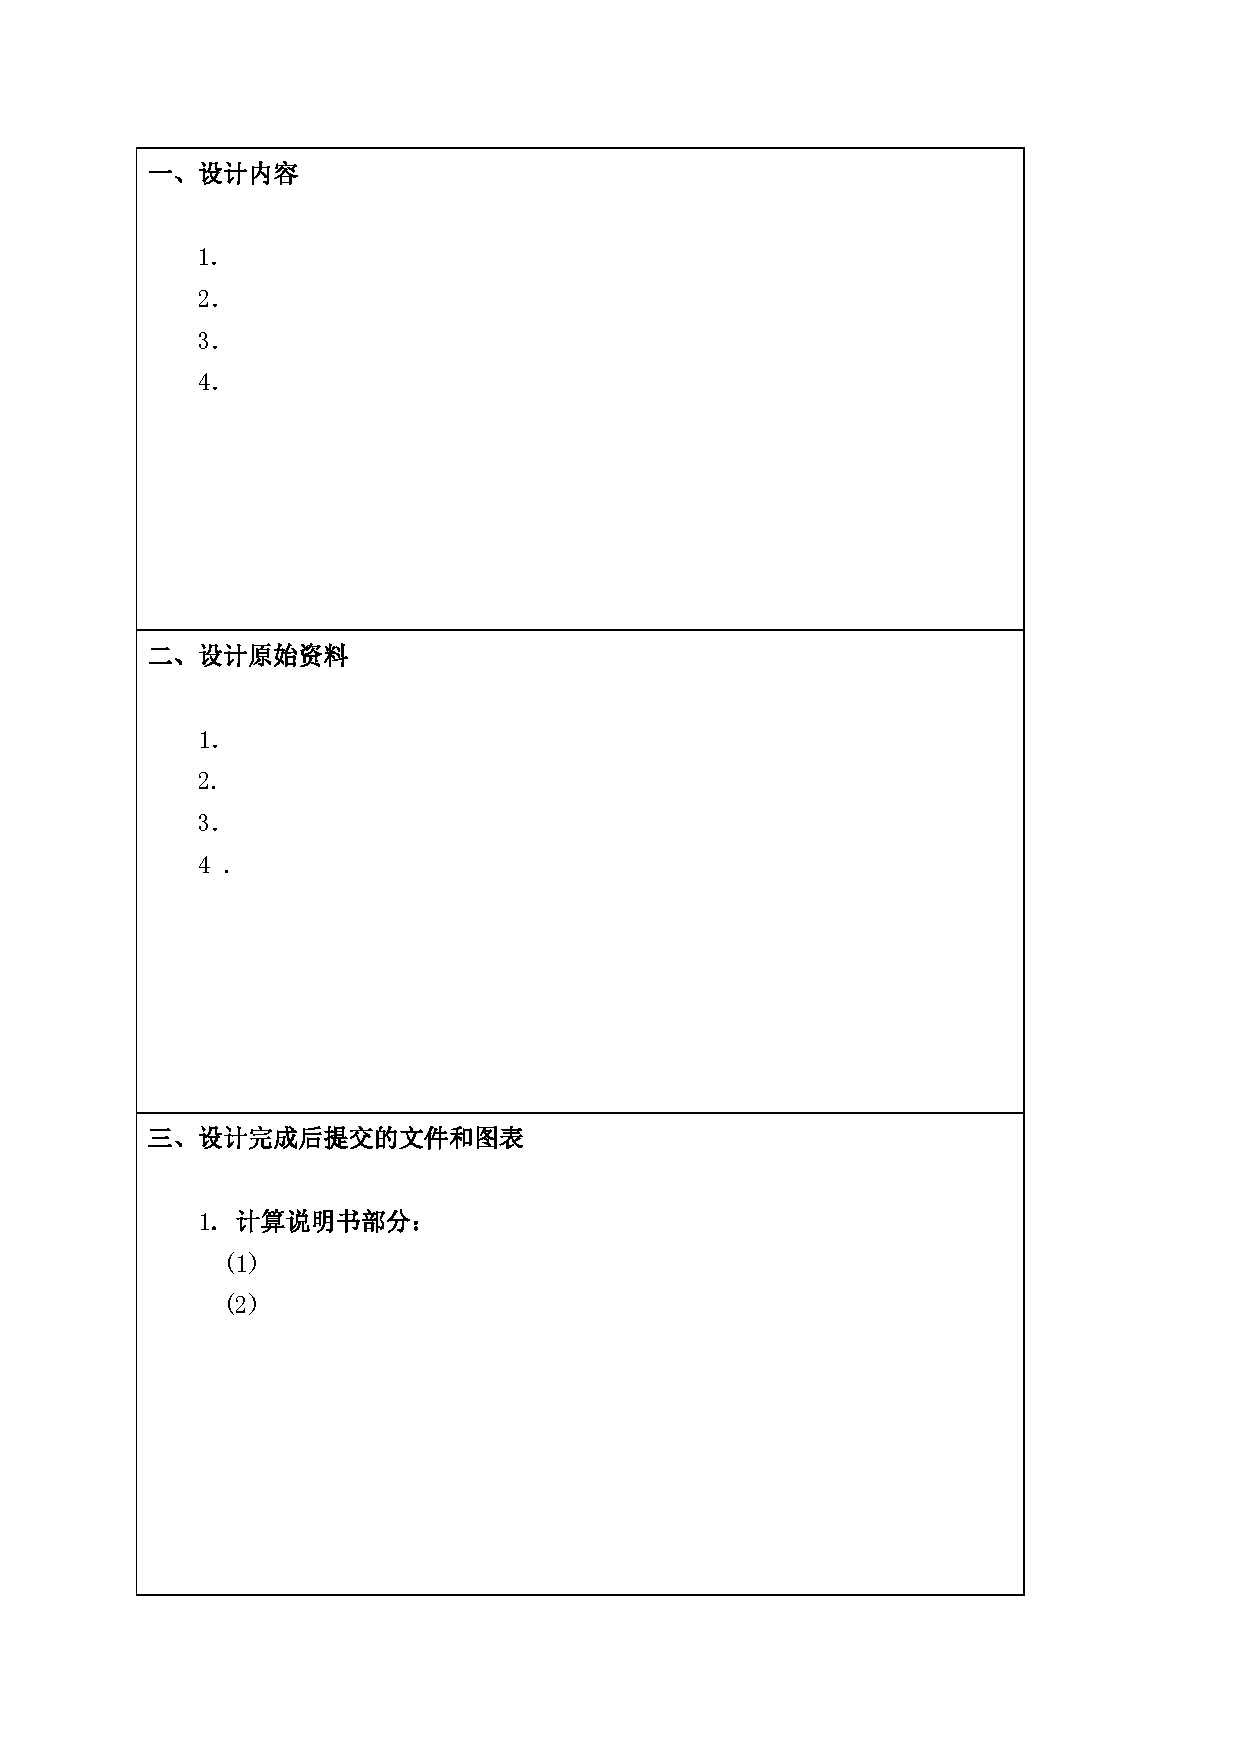
\includepdf[nup=1x1, delta=0mm 0mm,scale=1,pages={1-6}]{a3cover/frontpage.pdf}|,其中\latexinline|pages={1-6}|是你frontpage的页码范围。还有附件里的外文文献及翻译,也是用这种方法载入。还有\LaTeX{}分段缩进不用空格,直接回车两下,就是空一行

像这样,详细参考本文代码。公式、插图、表格下面段落也要空一行,否则不会缩进。但是如果遇见章节标题,就不用空行了,会自动缩进。
\subsection{免责声明}
\begin{myList}
\item 本模板的发布遵守\LaTeX{} Project Public License,使用前请认真阅读协议内容
\item 本模板的出发点是方便大家使用专业的高效的论文书写工具,其优点在于注重排版质量、命令规范、使用方便,符合论文撰写说明。但任何由于使用本模板而引起的论文格式审查问题均与本模板作者无关。
\item 任何个人或组织均可以本模板为基础进行修改、扩展,生成新的专用模板,但
请严格遵守\LaTeX{} Project Public License 协议
\end{myList}
\begin{figure}[htp]
\centering
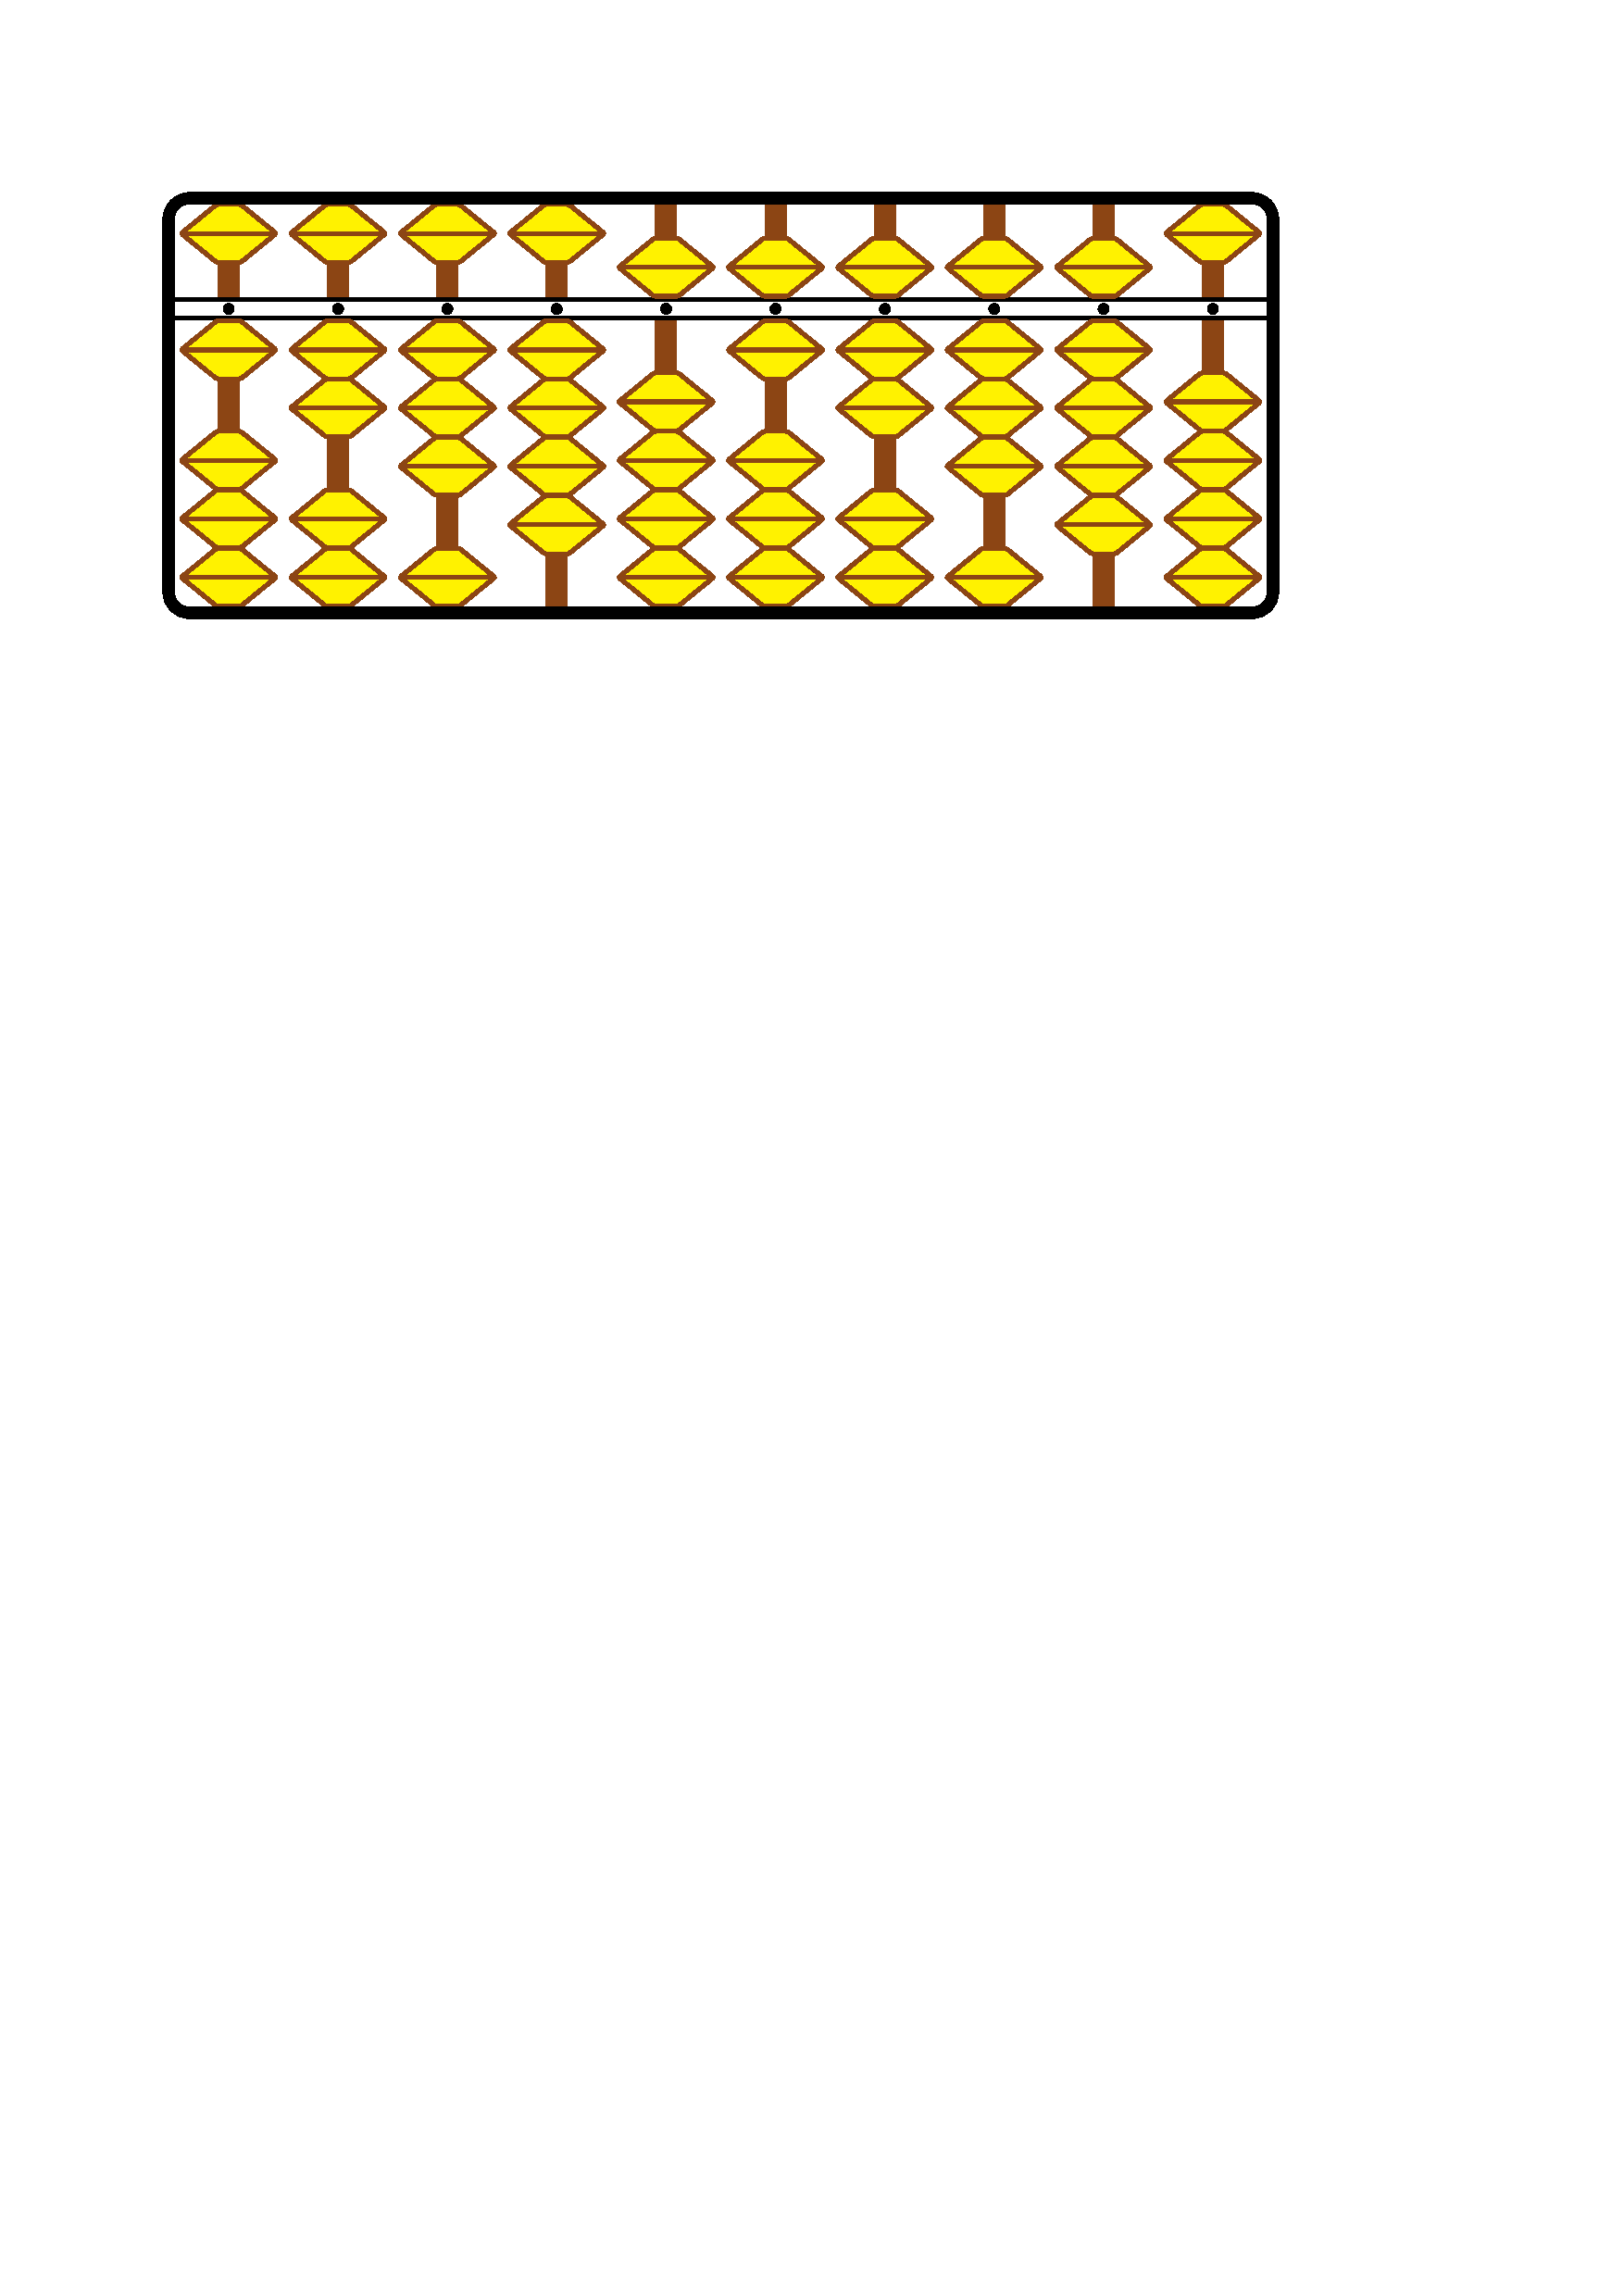
\includegraphics[width=5in]{soroban.pdf}
\caption{soroban宏包绘制的算盘}
\end{figure}

由于有些地方用\latexinline|itemize|不太合适,也用不上\latexinline|\subsubsection|这样的小小节,所以就把它改成下面的样子了。但是在每次使用前得先把计数器初始化为1,\verb|\setcounter|\verb|{shuzi}{1}|
\subsubsection{(题目(1))}
本章的主要内容与学校提供的Word模板中内容一致,图片与表格均采用原始设定大小,%
主要是为了说明格式的统一。%
但是,\LaTeX{}的一些禁则,专业排版的能力,对公式及文献的处理都是得天独厚的,%
我们不必刻意去追求与Word的完美匹配。而且你将会发现,用\LaTeX{}书写论文的美! %

\subsubsection{(题目(1))}
用户在使用中遇到问题或者需要增加某种功能,都可以和作者联系:
Tsingber Lee <xiaolee2520@gmail.com>
欢迎大家反馈自己的使用情况,能为长大本科生的作出一点点的贡献,也祝
长安大学的同学前程似锦。

\subsection{(1.1.2 题目)}
正文内容

正文内容
\begin{figure}[htp]
\centering
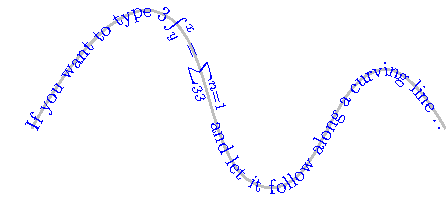
\includegraphics{followline.pdf}
\caption{followline}
\end{figure}

\begin{figure}[htp]
\centering

\includegraphics{shiliu.jpg}
\caption{世园会吉祥物}
\end{figure}

\section{1.2节题目}
正文内容

正文内容

\begin{table}[htp]
\centering
\caption{表 1.2 名称}
\begin{tabular}{|c|c|c|c|c|}
\hline
\makebox[2.07cm][0pt]{} & \makebox[2.07cm][0pt]{} & \makebox[2.07cm][0pt]{} & \makebox[2.07cm][0pt]{} & \makebox[2.07cm][0pt]{} \\
\hline
 & & & & \\
\hline
 & & & & \\
\hline
\end{tabular}
\end{table}
\subsection{题目}
\begin{figure}[htp]
\centering
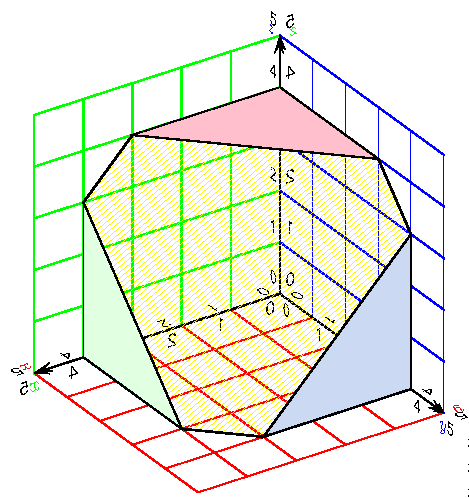
\includegraphics[width=5in]{pstricks-doc1.pdf}
\caption{空间立体}
\end{figure}
\subsection{题目}
正文内容

正文内容

\section{本文主要研究内容}
\begin{figure}[htp]
\centering
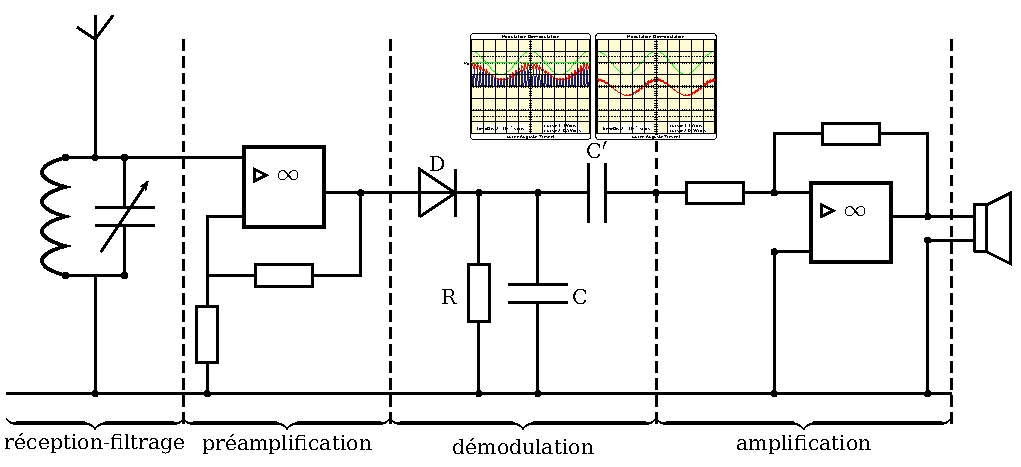
\includegraphics[width=5in]{pst-am-doc.pdf}
\caption{电路图}
\end{figure}

正文内容
\begin{figure}[htp]
\centering
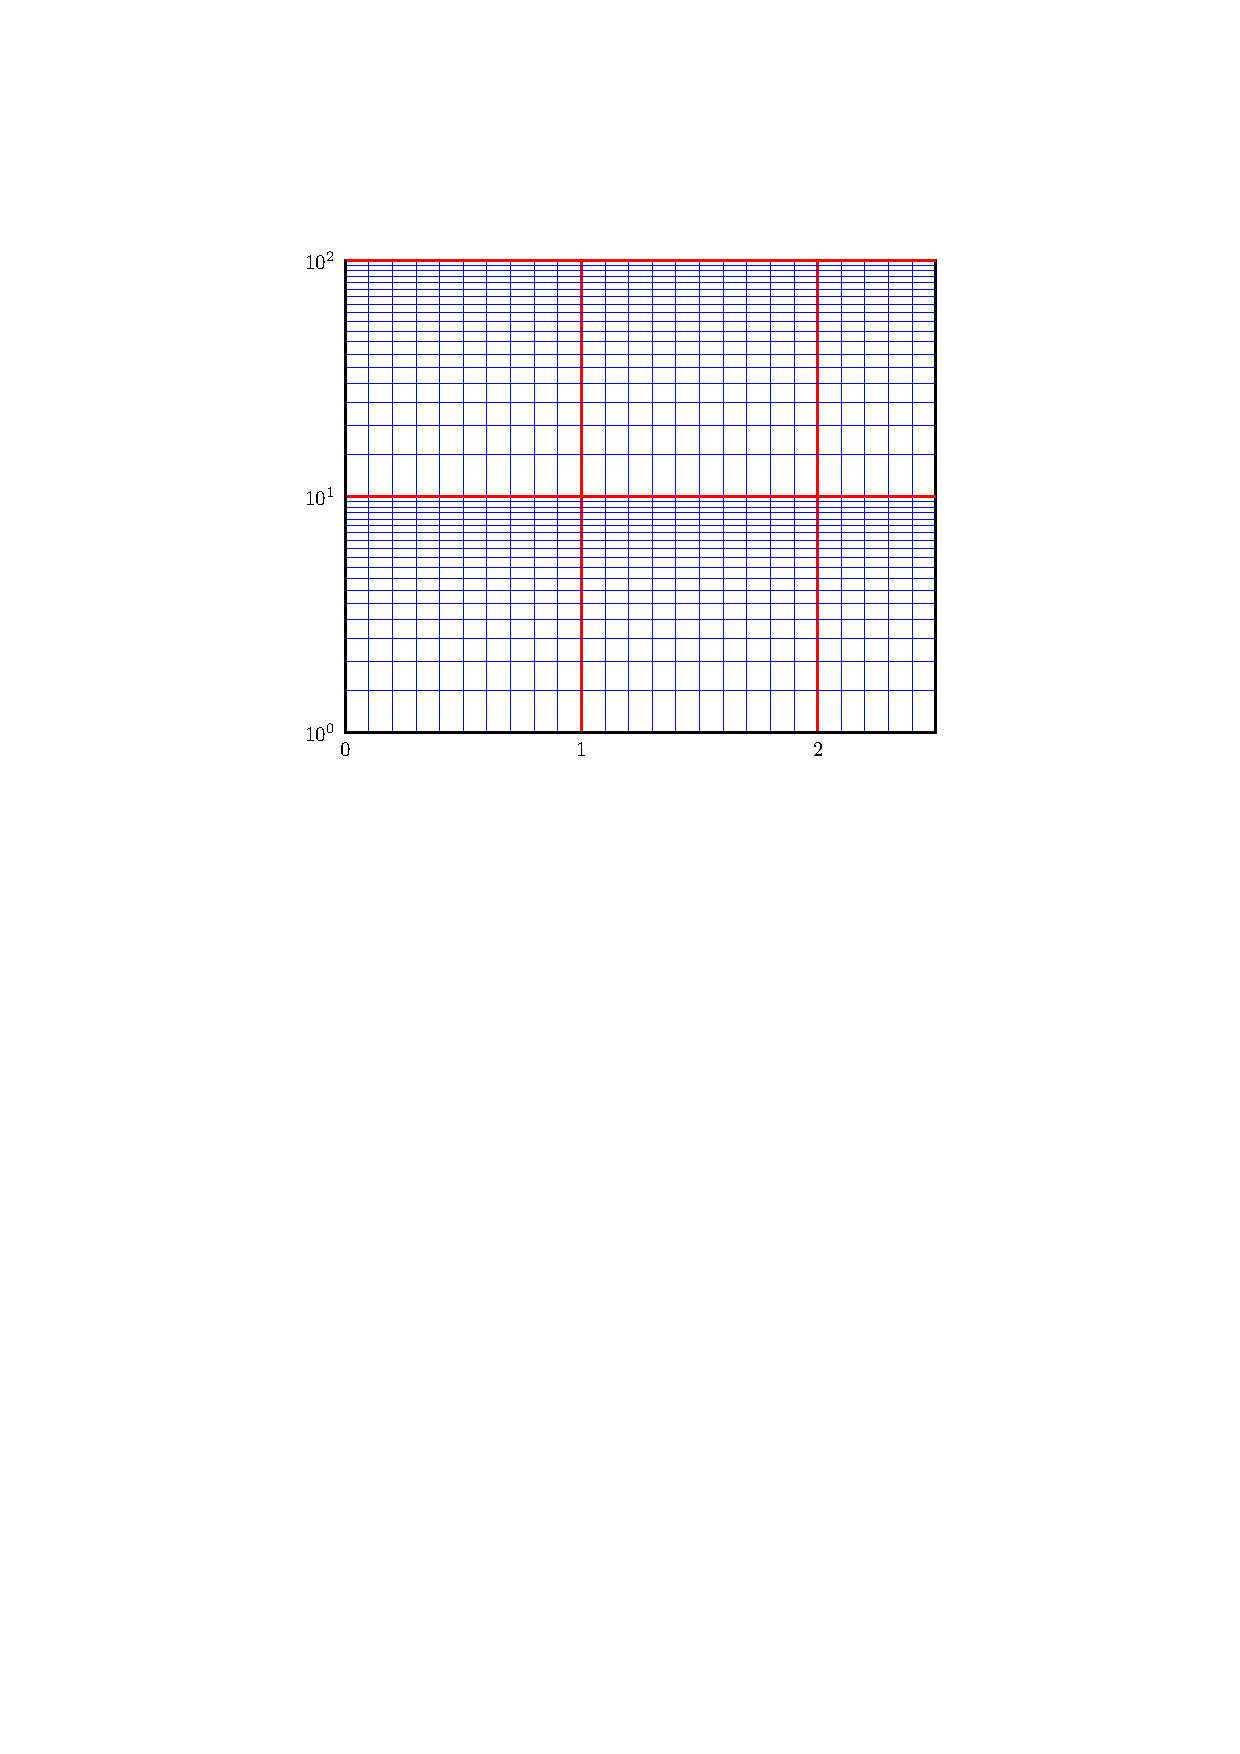
\includegraphics[width=4in]{pst-loglines.pdf}
\caption{对数坐标,在物理实验时可以用到}
\end{figure}

\begin{figure}[htp]
\centering
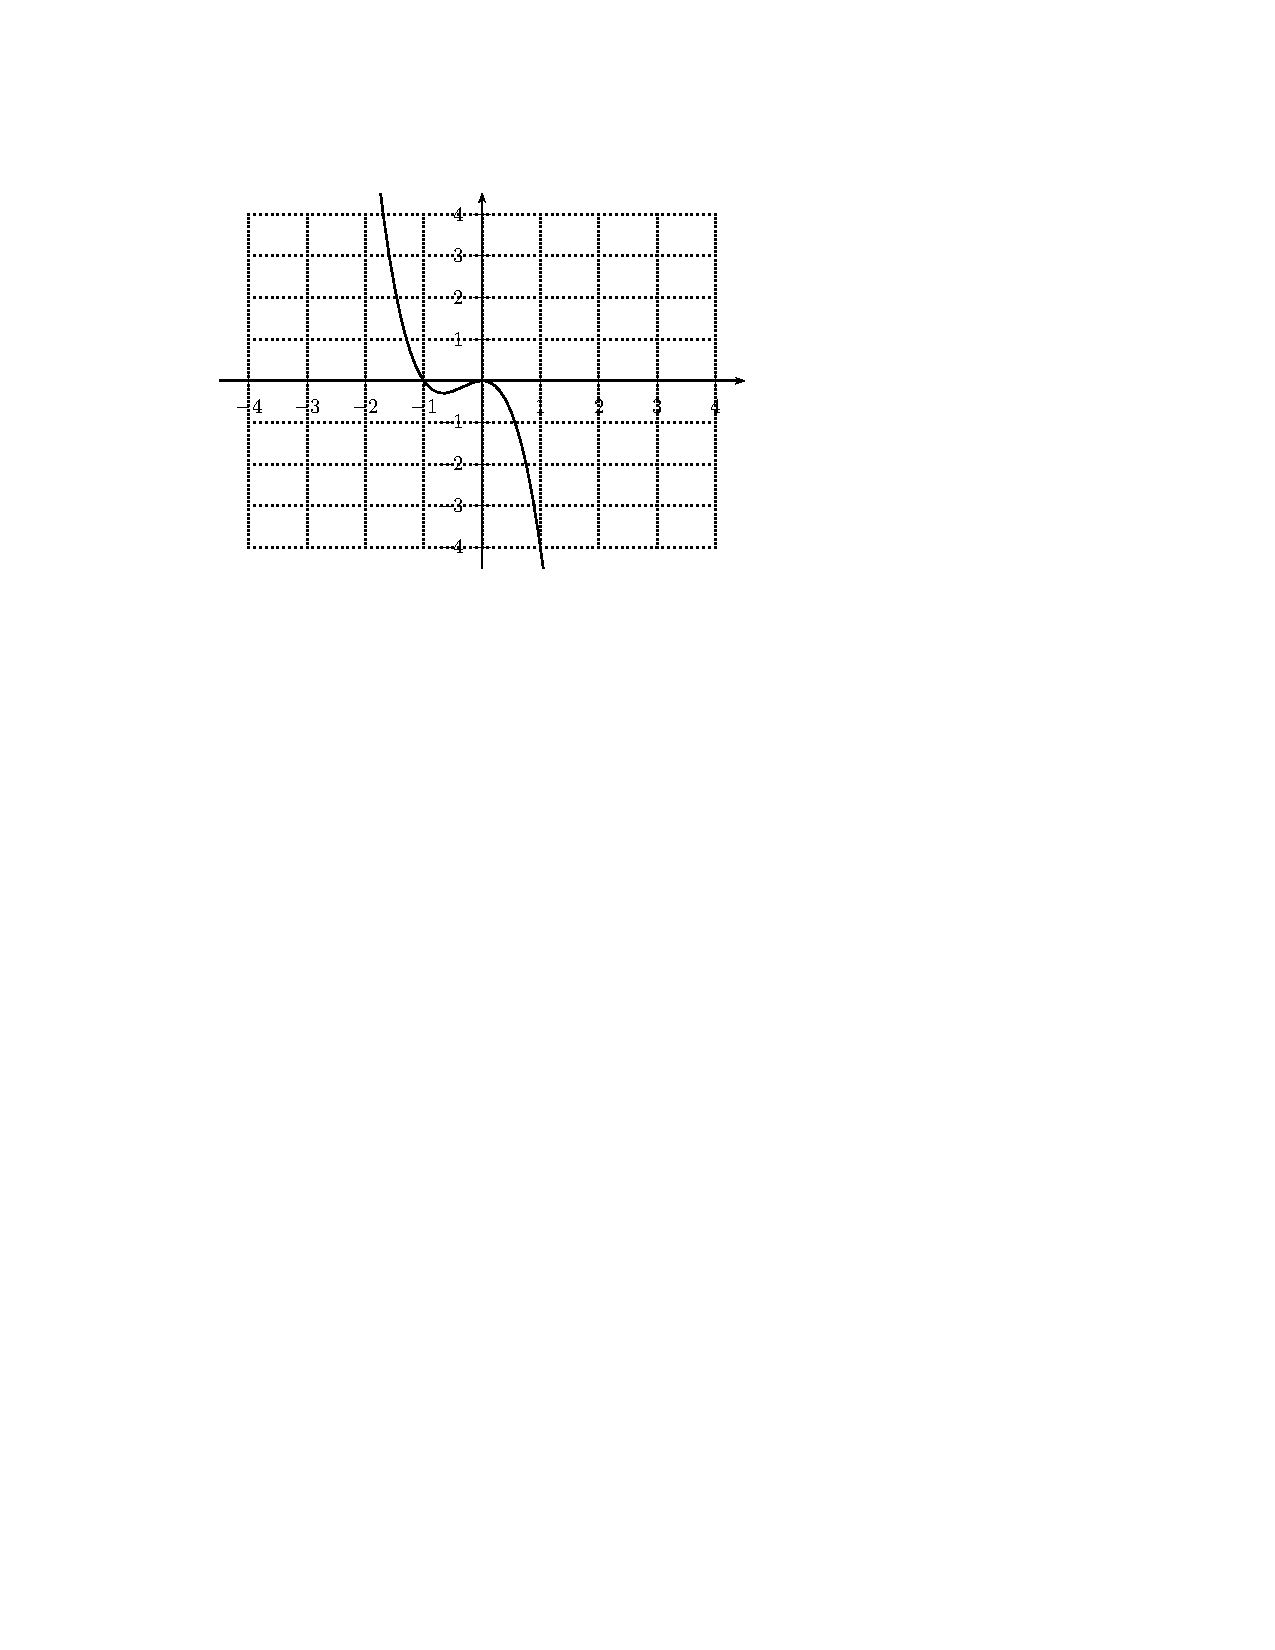
\includegraphics[width=4in]{graph.pdf}
\caption{二维坐标}
\end{figure}
\begin{figure}[htp]
\centering
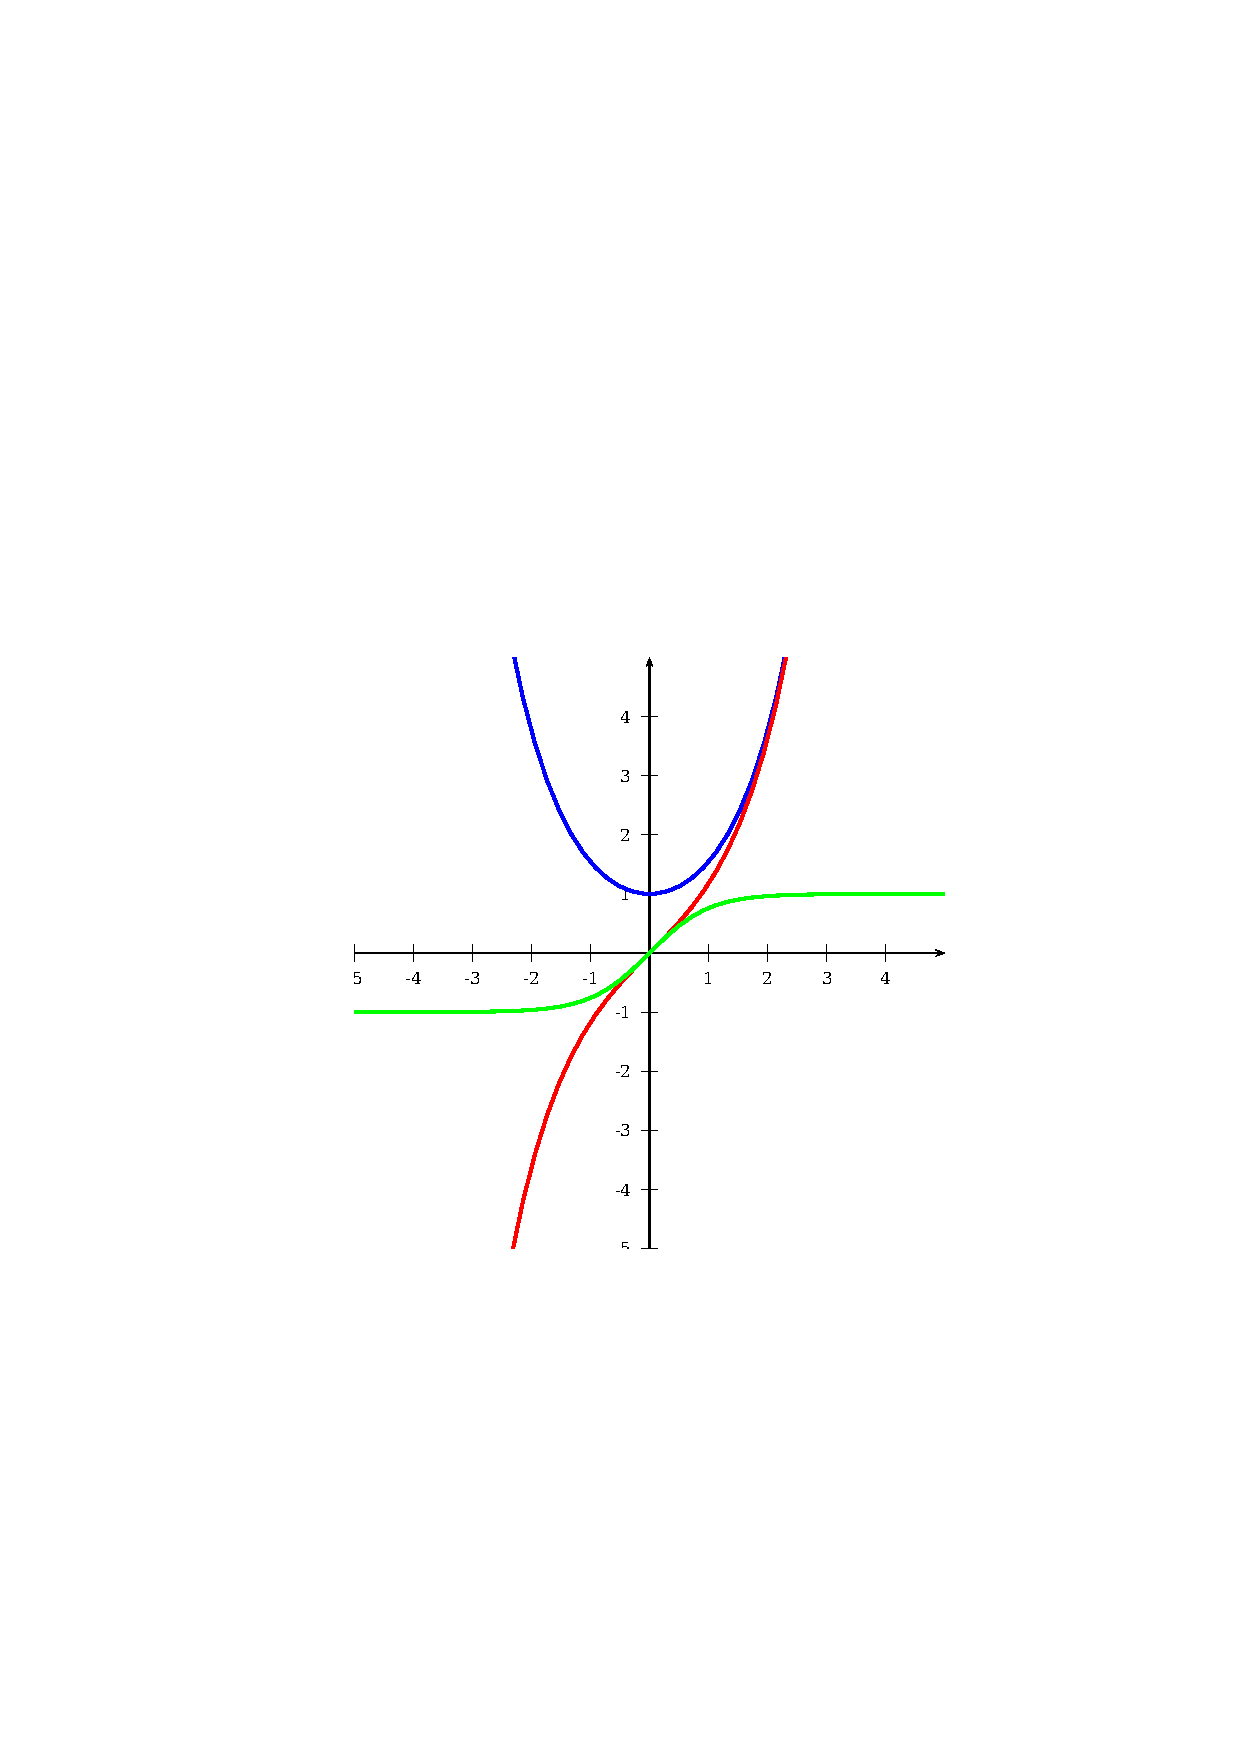
\includegraphics[width=4in]{pst-math-doc.pdf}
\caption{多个函数}
\end{figure}
\subsection{有意思的绘图宏包}
正文内容

\begin{figure}[htp]
\centering
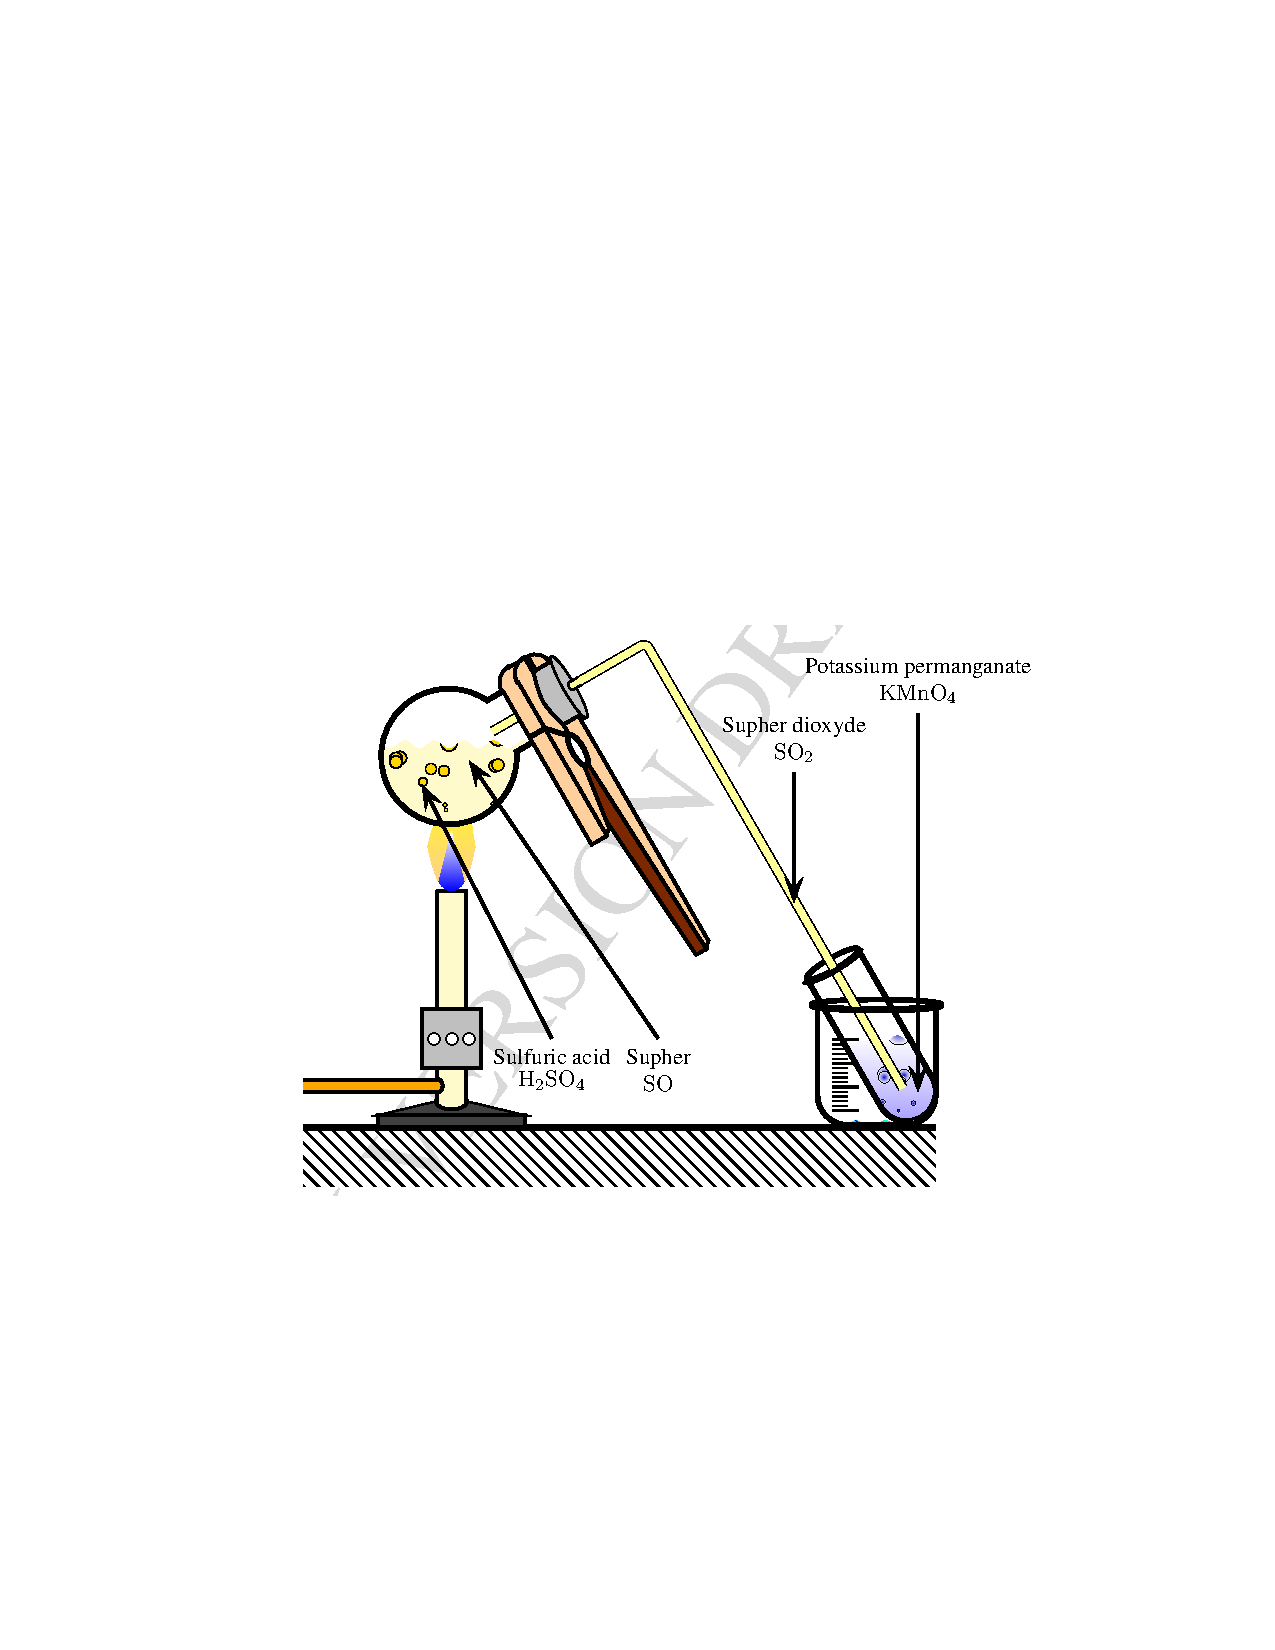
\includegraphics[width=3in]{pstricks-chemical.pdf}
\caption{pstricks宏包绘制的化学实验}
\end{figure}

\subsection{(1.3.2 题目)}
正文内容

正文内容

\begin{table}[H]
\centering
\caption{表 1.2 名称}
\begin{tabular}{|c|c|c|c|c|}
\hline
\makebox[2.07cm][0pt]{} & \makebox[2.07cm][0pt]{} & \makebox[2.07cm][0pt]{} & \makebox[2.07cm][0pt]{} & \makebox[2.07cm][0pt]{} \\
\hline
 & & & & \\
\hline
 & & & & \\
\hline
\end{tabular}
\end{table}
%htbp选项用来指定插图的理想位置,这几个字母分别代表here,top,bottom,float page,也就是就这里、页顶、页尾、浮动页(专门放浮动环境的单独页面)。我们可以使用这几个字母的任意组合,四个字母都写上表示放哪里都无所谓;一般不推荐单独使用h,因为latex自以为它的排版算法是最完美的,不愿意被束缚手脚。
\begin{figure}[htb]
\centering
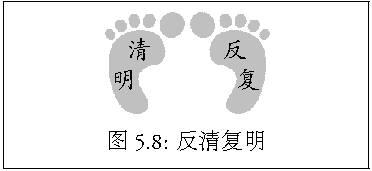
\includegraphics{lnotes2.pdf}
\end{figure}
本模版是根据长安大学毕业论文格式规范制作的\LaTeX{}毕业论文模
板。
本模板是基于国防科技大学的硕博士论文模板,并
按照长安大学毕业论文格式规范开发的\LaTeX{}论文模板,经过完善和修改,目
前已经基本满足了论文规范的要求,而且易用性良好,功能强大。不过,可能还存在着
一些问题,欢迎大家积极使用本模版,反馈遇到的问题,以便不断对其进行改进。
当然这个模板仅仅是一个开始,希望有更多的\TeX{er}能够参与进来,不断改进准确性、
易用性和较好的可维护性,造福需要的兄弟姐妹们。总体上来说,当前这个模板还是很
值得推荐使用的。

本模板的目的旨在推广\LaTeX{}这一优秀的排版软件在长大(尤其是数学相关专业)
的应用,为广大同学提供一个方便、美观的论文模板,减少论文撰写格式方面的麻烦。

\bigskip
Q: ``If you were young again, would you start writing \TeX{} again or would you
use Microsoft Word, or another word processor?"

A: ``I hope to die before I have to use Microsoft Word."

\medskip\hfill Harald K\"{o}nig asking Donald Knuth, T\"{u}bingen, 2 Oct 2001.
\begin{figure}[htp]
\centering
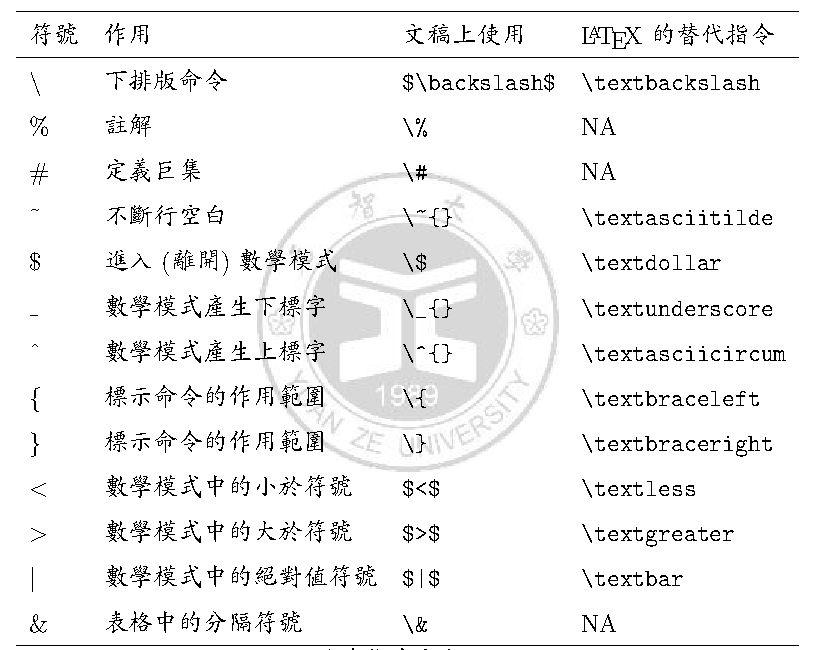
\includegraphics{fuhao.pdf}
\caption{無法直接在\LaTeX{}文稿裏使用的符號字元}
\label{fig:symble}
\end{figure}

图 \ref{fig:symble}的表格列出无法直接在\LaTeX{}文档中使用的符号\footnote{截图自\kai 元智大學光電工程研究所碩士論文}